\documentclass[a4paper,10pt]{article}

%%%%%%%%%%%%%%%%%%%%%%%%%%%%%%%%%%%%%
%% Select input file encoding:
%%   utf8   - UTF-8, nowadays standard on most operating sytems
%%   latin1 - ISO-8859-1
\usepackage[utf8]{inputenc}

%%%%%%%%%%%%%%%%%%%%%%%%%%%%%%%%%%%%%
%% Select language
%%
%\usepackage[ngerman]{babel}        % Deutsch, neue Rechtschreibung
\usepackage[english]{babel}       % English

\usepackage[T1]{fontenc}           % Font encoding (don't change!)
\usepackage{lmodern}               % Select Linux Modern Fonts (don't change)
\usepackage{sansmathfonts}         % Sans fonts in math environments
\usepackage{textcomp}              % fix 'missing font symbols' warning
\renewcommand{\rmdefault}{phv}     % Arial like (Helvetica)
\renewcommand{\sfdefault}{phv}     % Arial like (Helvetica)

%% graphics related packages
\usepackage{graphicx}              % needed to include graphics (don't change)
\usepackage{epstopdf}              % required to include eps files
%\usepackage{svg}                   % include svg files (requires Inkscape)
\usepackage[encoding,filenameencoding=utf8]{grffile} % allow utf8 file names in graphics

%%%%%%%%%%%%%%%%%%%%%%%%%%%%%%%%%%%%%
%% import packages for content
%%
\usepackage{listings}                           % for lstlisting and \lstinline|..|

\usepackage{hyperref}
%% Custom packages and definitions

% Mathematikumgebung
\usepackage{amsmath}
\usepackage{amssymb}
\usepackage{sansmath}

% tabularx -> bessere "tabular"-Umgebung
\usepackage{tabularx}

% Bessere Tabellenlinien
\usepackage{booktabs}


\usepackage[version=3]{mhchem} % Formula subscripts using \ce{}
\newcommand{\nox}{NO$_x$} % our abbreviation

\newcommand{\red}[1]{\textcolor{red}{#1}} %easy red text


\title{PCFC QM Subgroup:\\An introduction to \textsc{MESS}}%[Introduction to \textsc{MESS}]
\author{Mark E. Fuller\footnote{\href{mailto:fuller@pcfc.rwth-aachen.de}{fuller@pcfc.rwth-aachen.de}}}


%\logo{\includegraphics[height=8mm]{logos/logo}} % will replace the default logo

% official institute logo offset correction
%\logo{\vskip-3.5mm\includegraphics[height=12.5mm]{logos/rwth_mentoring_rgb.eps}\hspace{-2mm}} % optionally
%\logo{\vskip-2mm
\includegraphics[width=45mm]{logos/PCFC.png}\hspace{-2mm}} % optionally


\begin{document}
\maketitle
\section{Introduction}
\subsection{What is \textsc{MESS}?}
  \begin{itemize}
   \item \textsc{MESS} is the \textbf{M}aster \textbf{E}quation \textbf{S}ystem \textbf{S}olver (\href{https://doi.org/10.1021/jp4060704}{Publication}\cite{Georgievskii.2013}), a component of the \textsc{PAPR} suite of chemical kinetics codes
    \begin{itemize}
     \item Developers: Y. Georgievskii, C. F. Goldsmith, J. A. Miller, M. P. Burke, and S. J. Klippenstein 
     \item \textsc{PAPR}: \url{https://tcg.cse.anl.gov/papr/codes/mess.html}
    \end{itemize}
   \item Conformers on a potential energy surface are connected via transition states
   \item Ab initio calculations provide necessary input information to calculate partition functions and determine rates via transition state theory (TST)
  \end{itemize}


\subsection{\ce{H2N1O2} Potential Energy Surface}
Consider simple PES as example system (\href{https://doi.org/10.1016/j.proci.2018.06.208}{Publication}\cite{Fuller.2018})
  \begin{itemize}
   \item System consists of three kinds of nodes (conformers):
    \begin{itemize}
     \item \textsc{Bimolecular}: a pair of fragments which are lumped together, \textit{e.g.} \ce{H}+\ce{HNO2}
     \item \textsc{Well}: a unimolecular intermediate, \textit{e.g.} \ce{HONOH}
     \item \textsc{Barrier}: a transition state (TS) between two wells/bimoleculars
    \end{itemize}
   \item Each conformer is described by its geometry and frequencies and (relative) energy
  \end{itemize}
%  \columnbreak
  \begin{figure}
    \centering
    %tex file to generate this figure in figures folder
    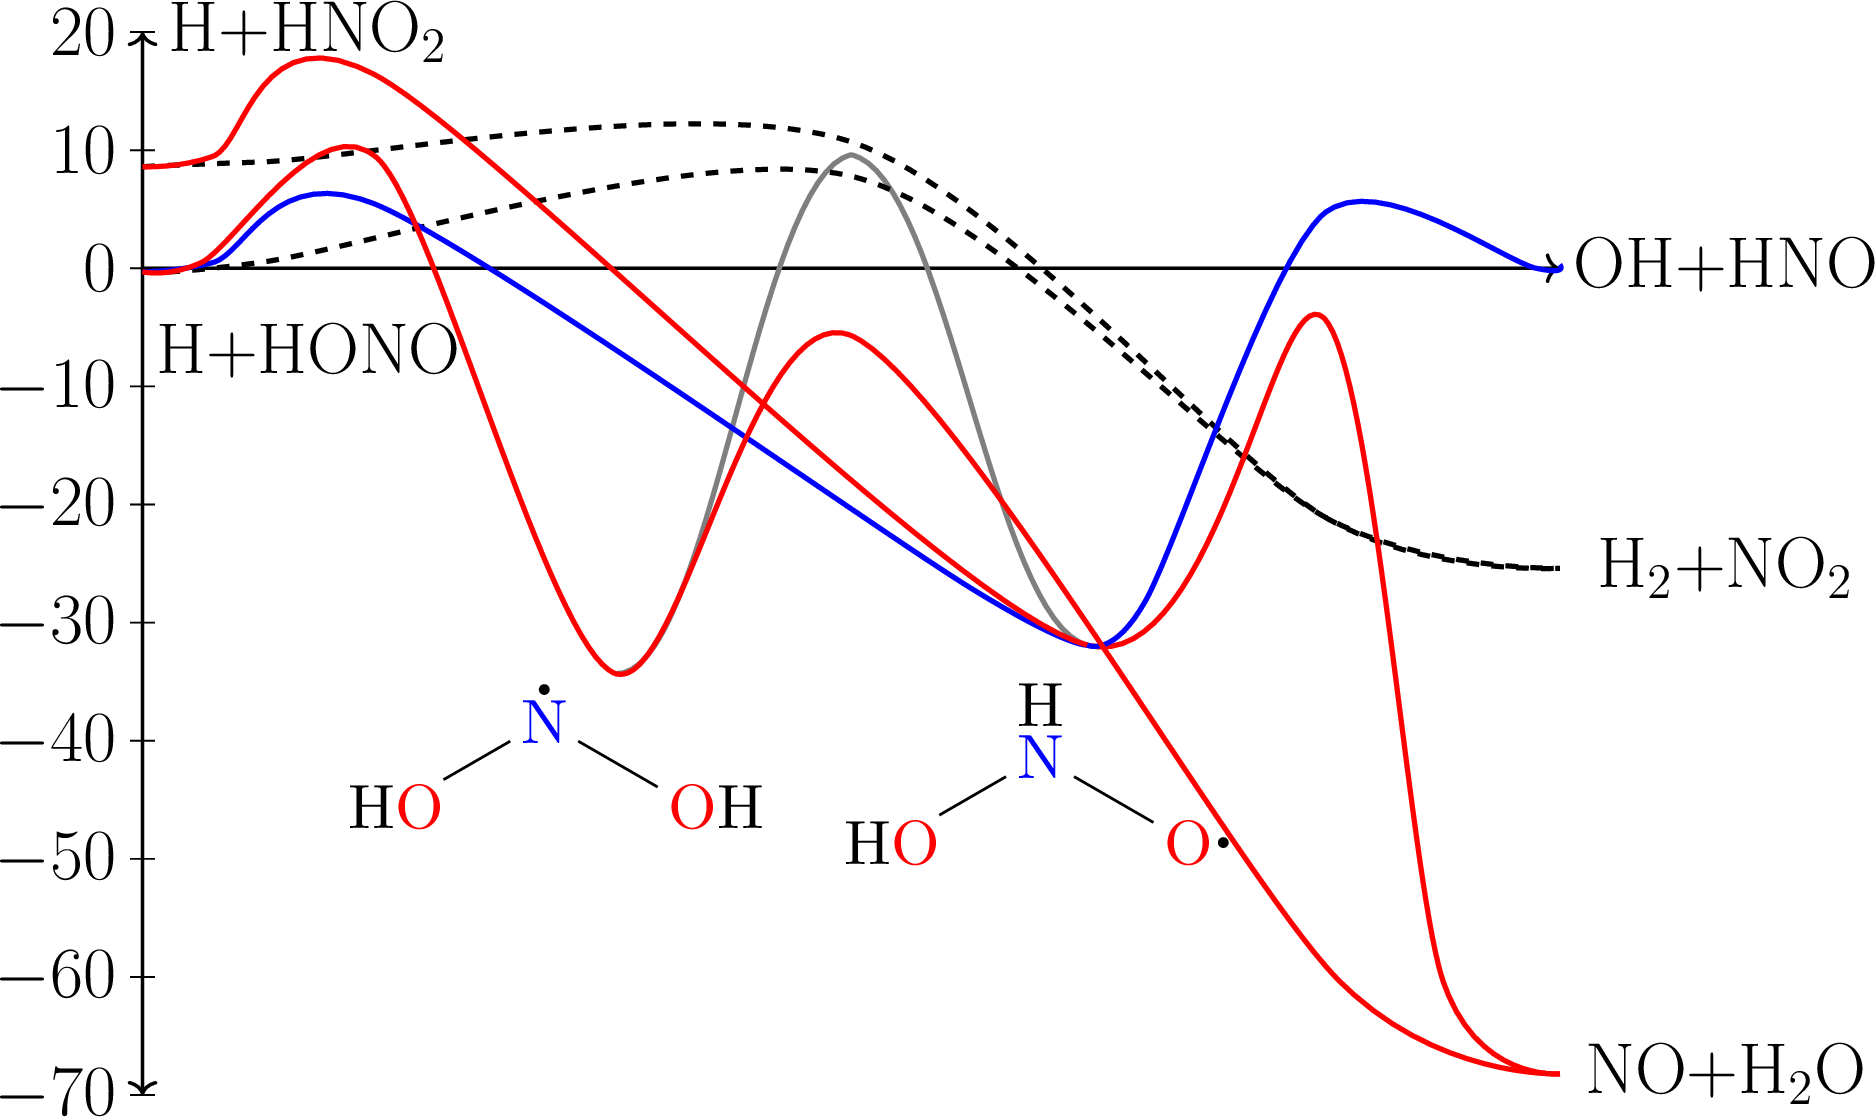
\includegraphics[width=0.6\linewidth]{figures/PES_H_HONO_1_lumpHONO.png}
  \end{figure}
%\end{multicols}


\section{MESS Input File}
% /home/fuller/Documents/PCFC/Pubs_Pres/QMsubgroup/20200512_MESS/MESS_Version0/Current/h2no2_b2plypd3_ccpvtz_lhono_0.inp
% \lstinputlisting[language=Python, linerange={37-45,48-50}]{source_filename.py}
% \lstinputlisting[language=Python, firstline=37, lastline=45]{source_filename.py}
%
% This requires the package listings
% 
% Slides containing lstlisting environments, \lstinline|..| or \verb|..|
% the option "fragile" must be provided!  /home/fuller/Documents/PCFC/Pubs_Pres/QMsubgroup/20200512_MESS/
% 


\subsection{Input file overview}
  \begin{itemize}
   \item Global section (unnamed header) specifies parameters for solution of the master equation
   \item Specify temperatures, pressures, calculation parameters
   \item Two major choices for calculation method
    \begin{itemize}
     \item \textsc{direct}: fuller, more expensive calculations (not so good at low temperature)
     \item \textsc{low-eigenvalue}: assume which eigenvalues are chemical and which are relaxational, numerically cheap, not accurate at high temperatures
    \end{itemize}
   \item \textsc{Model} definition follows and begins with collision parameters
   \item All conformers are then described to define system
  \end{itemize}


\subsubsection[fragile]{Header Information}
  \lstinputlisting[lastline=22]{MESS/h2no2_b2plypd3_ccpvtz_lhono_0.inp}


\subsubsection[fragile]{Bimolecular Input}
  \lstinputlisting[firstline=24,lastline=60]{MESS/h2no2_b2plypd3_ccpvtz_lhono_0.inp}


\subsubsection[fragile]{Well Input}
  \lstinputlisting[firstline=248,lastline=284]{MESS/h2no2_b2plypd3_ccpvtz_lhono_0.inp}


\subsubsection[fragile]{Barrier Input}
  \lstinputlisting[firstline=288,lastline=323]{MESS/h2no2_b2plypd3_ccpvtz_lhono_0.inp}


\subsection{Generating \textsc{MESS} Input Blocks}
  \begin{itemize}
   \item While you could, it is tedious and error-prone to write input files manually
   \item The utility program \textsc{writemess} reads a \textsc{Gaussian} output (log) file and writes a conformer template
   \item Optionally, hindered rotors (\textsc{Gaussian} log files) and energy from a single-point calculation (\textsc{ORCA}, currently) may also be added and written concurrently
  \end{itemize}


\section{Getting Results}
\subsection{Job Submission and Output}
  \begin{itemize}
   \item Assuming everything is installed correctly, job submission on the HPC with slurm is simple: we call \textsc{mess} on the input file
   \begin{itemize}
    \item If we have an input file for a network of bimoleculars, wells, and barriers, then we call \textsc{mess} on the input file
    \item For two bimoleculars connected by a single transition state, we call \textsc{abstraction} on the input file
   \end{itemize}
   \item A log file and output file will be generated by \textsc{MESS}
   \item Output file can be split into three sections:
    \begin{enumerate}
     \item System network at the top
     \item Rate tables at each temperature and pressure condition
     \item Rate tables for each species pair
    \end{enumerate}
   \item The output file requires conversion to a recognized format for inclusion in chemical kinetic mechanisms
  \end{itemize}


\subsection{Fitting the Output}
  \begin{itemize}
   \item A function to fit the output data to pressure-dependent, modified Arrhenius expressions is posted on the \textsc{MESS} webpage, \url{http://tcg.cse.anl.gov/papr/codes/mess/mess_aux/mod_arr.tgz}
   \item You will likely need to make some small changes for your specific system, but this will output \textsc{CHEMKIN}-format \textsc{PLOG} fits for all of the conformer pairs
  \end{itemize}


\section{Additional Resources}
  \begin{itemize}
   \item The \textsc{MESS} manual: \url{http://tcg.cse.anl.gov/papr/codes/mess/messmanual_3_23_16.pdf}
   \item More examples to run and test: \url{http://tcg.cse.anl.gov/papr/codes/mess/MESS_Examples.tgz}
  \end{itemize}



\bibliographystyle{elsarticle-num} 
\bibliography{references,ownpubspres}

\end{document}
